\chapter{Software Resilience against Dense Errors}
\label{c:resilience}

\section{Resilience in a Nutshell}
From Example~\ref{exmp.avi} to \ref{exmp.satt} in the previous section, it is easy to see the common paradigm of error recovery in software systems.  

\begin{quote}
When errors are detected, a recovery mechanism will be activated to avoid failures and try to get back to normal execution. 
\end{quote}

Moreover, such a recovery mechanism usually needs to operate under the assumption that more errors may also happen during the recovery process.
In practice, system designers have already implemented many defensive modules, e.g., exception handlers, which are certainly good candidates for the recovery segments.  
Thus, the recovery scheme we discuss is likely to have arisen in an ad-hoc fashion as a natural concept when software architects and programmers designed recovery mechanisms for critical software.  

The vast state spaces of critical systems make an automated support for and a solid foundation of evaluating design alternatives particularly valuable. 

In the following, we will use the examples from the previous subsection as a motivation for defining a new game, called {\em safety resilience game}, between the recovery mechanism (the protagonist) and the error-injecting agent (the antagonist).  
The game is specified with a set $F$ of failure states, a set $S$ of safe states (the safety region), the moves by the antagonist to inject errors, and the resilience level $k$ that the designers want to achieve. 
The objective of the protagonist is to identify a control strategy so that the whole system can achieve the prescribed level (or the highest level) $k$ of resilience for safety region $S$ (a set of states) and failure state set $F$.  

The game is played round by round. 
When the antagonist issues an error move, 
the play may be deflected into a recovery segment.  
If there are no more than $k-1$ errors in the recovery segment, 
then a $k$-resilient control mechanism must direct the recovery segment
to end at a safe state. 
The above observation suggests that 
a safety region can be abstracted as a fixed point 
to the recovery procedure 
that transforms a safe state to another safe state via the recovery segment 
with at most $k-1$ errors. 
Conceptually, a fixed point to a procedure $f(x)$ is a set $S$ of elements 
in the domain of $x$ such that $S=\{f(x)\mid x\in S\}$.  
To calculate the fixed point of the recovery procedure, 
we can use the greatest fixed point algorithm.  
The idea is to start from a superset of the recovery procedure fixed point. 
For convenience, we call a superset of the fixed point a {\em pseudo fixed point} 
({\em PFP}).  
Then we iteratively check every state $q$ in the PFP and eliminate 
$q$ from the PFP if, after at most $k$ errors from $q$, 
the recovery mechanism either cannot avoid failure or 
cannot direct the system back to the PFP. 
As the iterative checking and elimination goes on, 
the PFP will shrink and eventually stabilize.
Note that its size is always finite, 
since the initial PFP must be no bigger than $Q$.  
The final PFP is then a greatest fixed point to the recovery mechansim for 
$k$-resilience and is the legitimate safety region.  
 

This recovery procedure can be illustrated as in Figure~\ref{fig.sfrch} 
for resilience to $2$ errors.  
\begin{figure}[t]
\begin{center}
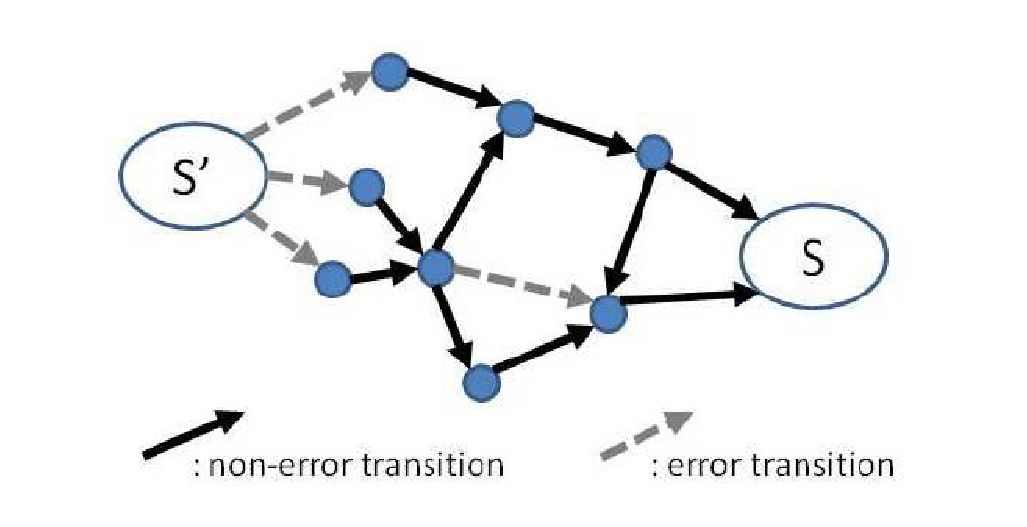
\epsfig{file=rseg.eps,width=60mm}
\caption{Illustration of the recovery operation}
\label{fig.sfrch} 
\end{center}
\end{figure}  
In this figure, the states in set $S'$ are computed  
as the precondition of states in $S$ through those transitions in the figure.  
Each path from $S'$ to $S$ is a recovery segment. 
$S$ and $S'$ may overlap.  
The blue circles represent states in the recovery segments.  
If we calculate $S'$ out of $S$, 
then, for each state $q'\in S'$, we can find a path from 
$q'\in S'$ via a path in the recovery segment to another state $q\in S$.  
The maximal number of errors in a recovery segment is 2.  
Thus the protagonist has a strategy to recover from errors in $S'$ to $S$ 
even when 2 errors happen in the corresponding recovery segment.  
When $S'=S$, then $S$ is a fixed point to the precondition 
operator through the recovery segments in the figure.  

Now we formally define the concept that we explained with Figure~\ref{fig.sfrch}.  

\begin{definition}{\bf ($k$-safety):} 
\label{k-safe}
Given a $k\in\nnneg$, 
a state $q$ is called \mbox{$k$-safe} with respect to 
a safety region $S\subseteq Q\smallsetminus F$ of non-failure states, 
denoted $q\in\safe_k(S)$, if there 
is a strategy for the protagonist to guarantee that 
we can reach back to $S$ from $q$, provided that
the overall count of errors is at most $k$.
\qed 
\end{definition}

However, the definition can be subtle in its interpretation.  
Specifically, the ability to stand against one wave of $k$ errors 
is not the same as that against repeated recovery 
from waves of $k$ errors.  
If the recovery mechanism is not designed properly, 
the system may gradually lose a bit of control after each wave of $k$ errors 
and eventually degrade to system-level failure. 

\begin{example} 
{\bf (Fault-tolerant computer architectures):}  
Consider Example~\ref{exmp.avi} with $2k+1$ processor copies, with the objective to maintain majority checks and to identify the bad processors. 
Indeed, according to the first, na\"ive solution, any safe state with a recovery strategy to $Q\smallsetminus F$ is good.   
After $k$ processor copies fail, the majority checks are still capable to maintain the correctness of the combined behavior to follow the design of the original system.
There seems to be nothing to do after $k$ errors.  
Thus, na\"ively, we can choose those states as the safety region if, at those states, majority checks still work.

However, there is no expectation that the system will be able
to recover at any point in the future into a situation where it can bear 
another wave of $k$ errors.   
It will fail and lose the function of majority checks just after one more error.  
In contrast, in this work, we aim to propose a dense error resilience criterion that 
given no more errors for enough time to allow recovery, 
the system will eventually recover to resilience to $k$ dense errors again. 
%Note that `enough time' is a system parameter that refers to the time required for recovery, provided no further errors occur.
\qed 
\end{example} 

To look at this issue in more detail, 
please consider the transition system with four states, 
including a single failure state
(state $4$, marked by a double line) shown in Figure~\ref{fig:example}.
The controlled transitions are depicted as black solid arrows, 
the error transitions are depicted as red dashed arrows.
For $S=Q\smallsetminus F=\{1,2,3\}$, all states in $S$ are in $\safe_0(S)$.
For all $k \geq 1$, we have $\safe_k(S)=\{1,2\}$:
the protagonist can simply stay in $\{1,2\}$ 
during the safety phase of the game, and once the antagonist 
plays an error transition, the game progresses 
into the recovery segment, where the protagonist's objective 
is satisfied immediately.
This outlines the difference between $k$-sfrch-ty and 
the linear time property
of being able to repeatedly tolerate waves of up to $k$ errors, 
which would only be satisfied by states $1$ and $2$ for 
$k = 1$, and only for state $1$ for $k = 2$.

\begin{figure}[t]
\begin{center}
\psset{xunit=26mm,yunit=7mm}
\begin{pspicture}(0,-.15)(3,1.4)
% \pnode(0,.6){0}
\rput(0,0){\circlenode{1}{$1$}}
\rput(1,0){\circlenode{2}{$2$}}
\rput(2,0){\circlenode{3}{$3$}}
\rput(3,0){\circlenode[doubleline=true]{4}{$4$}}
% \ncline{->}{0}{1}
\nccircle{->}{1}{.35}
\nccircle{->}{2}{.35}
\nccircle{->}{3}{.35}
\ncarc[linecolor=red,linestyle=dashed]{->}{1}{2}
\ncarc{->}{2}{1}
\ncarc[linecolor=red,linestyle=dashed]{->}{2}{3}
\ncarc{->}{3}{2}
\ncline[linecolor=red,linestyle=dashed]{->}{3}{4}
\end{pspicture}
\end{center}
\caption{\label{fig:example} An example for calculating $\safe_k$}
\end{figure}

This difference raises the question 
if the rules of our game are depriving the antagonist 
of some of the $k$ errors that she should intuitively be allowed to insert in a wave.
The answer is that this is not the case 
if we use any fixed point of $\safe_k$ as $S$.
In this case, the protagonist would regain the capability to endure a wave of $k$ errors when reaching a safe state after recovery.
Instead of depriving the antagonist, 
one could say that we reset the number of errors in any recovery 
segment that the antagonist can inject to $k$.
Thus such a fixed point of $\safe_k$ should consist of 
states, from which we can use a control mechanism to fend off 
repetitive waves of $k$ dense errors in the recovery segments.  
For convenience, we call states in such a fixed point of $\safe_k$  
the $k$-resilient states.

For a state to be in $\safe_k(S)$, 
the system (protagonist) has a strategy to recover to $S$, 
given that a long enough execution commenced 
without another round of $k$ errors happening.
We say that two successive errors are in the same 
\emph{group of dense errors} 
if the sequence of states separating them 
was not long enough for recovery to the safety region.
Vice versa, if two successive errors are far enough apart 
such that the protagonist can guarantee recovery in this separation, 
then they do not belong to the same group.

To check whether recovering to $S$ by the protagonist (the fault-tolerance mechanism)
is always possible, provided that at most $k$ errors occurred during 
a recovery segment, observe that nesting 
$\safe_k$ once, i.e., $\safe_k(\safe_k(\cdot))$, corresponds
to tolerating up to two rounds of up to $k$ dense errors, and so forth.
Thus, for $S$ to be a target of recovery for $k$-resilience, 
$S$ must be a fixed point of the operator
$\safe_k$ from Definition~\ref{k-safe}, or, equivalently, 
$S=\safe_k(S)$ must hold.  
Moreover, if $S$ is the greatest fixed point to $k$-resilience, then we we can apply 
$\safe_k()$ any number of times to $S$ and still obtain $S$.  
Computationally, the greatest fixed point of $\safe_k$ can be constructed as 
by executing  
\begin{center} 
$\safe_k(\safe_k(\safe_k(\ldots\ \safe_k(S\big)\ldots)))$,
\end{center}  
using a sufficiently deep nesting that a fixed point is reached.

Note that this fixed point $x$ to $x=\safe_k(x)$ is what we are really interested in, 
while $\safe_k(S)$ for a given $S$ is an intermediate result that does not 
guarantee survival of the systems after waves of dense errors.
If this greatest fixed point
$$R = \bigcup\{X \subseteq S \mid X = \safe_k ( X )\}$$ is non-empty, 
the protagonist's strategy for 
the fixed point (guaranteeing eventual recovery 
to a state in the fixed point within no more than $k$ errors, i.e., $k$-resilience) 
can be used to control the recovery mechanism, 
constraining its transitions to follow its winning strategy.

As explained in the introduction, there can be several natural control problems in our safety resilience game.
First, the system designers may want to know whether the chosen safety region $S$ can be supported by the recovery mechanism for resilience level $k$.  
Second, they may want to get design support for choosing the safety region for achieving resilience level $k$.  
Finally, they may want to know the maximal resilience level that they can achieve. 

we will explain the algorithm for constructing $\safe_k(\cdot)$ and evaluating $k$-resilient states.


\section{Safety resilience games}
A system is $k$-resilient if it
can be controlled to tolerate infinitely many groups of up to $k$ dense errors, 
provided that the system is given enough time to recover between these groups.
As we have explained, in systems developed with defensive mechanism against errors,  
when errors are detected, recovery procedures should be activated.  
The major challenge is to decide given a set of failure states and a safety region,
whether 
the recovery mechanism can support a resilience level required\label{reply1.prescribed.2.required} by the users. 
Our goal is to develop techniques with a solid foundation to 
assist the system designers in evaluating the resilience of their systems, 
to synthesize the controller strategy for the required resilience level, and 
to achieve the maximal resilience level. 


We now formally define the safety resilience game played between a 
system (the protagonist) and an error-injector (the antagonist).  
Initially, the two players are given a 2-player concurrent game structure $\calk$,  
a pebble in $r$,  
a set $F\subseteq Q$ of failure states, and 
a safety region $S\subseteq Q\smallsetminus F$. 
Then the recovery region consists of states in $Q\smallsetminus (F\cup S)$.  
The two players together make decisions and move the pebble from state to state.   
The antagonist tries to deflect a play into $F$ by injecting sufficiently many errors, while
% On the other hand, 
the protagonist tries to avoid that the pebble reaches $F$. 
To achieve this, the protagonist can use the recovery region as the safety buffer and try to 
get back to $S$ as soon as the play is deflected from $S$ 
to the recovery region.  
If a system is resilient to $k$ errors, then it means that 
the protagonist can handle up to $k-1$ errors while in the recovery region.  
Thus when checking whether a system is resilient to $k$ errors, 
we only need to check those recovery segments with no more than $k-1$ errors. 

In the following, we formalize the concept.  

\begin{definition} \label{def.srgs} 
{\bf (Safety resilience game structure):} 
Such a structure is a pair $\langle \calk, F\rangle$ with the following 
restrictions. 
\begin{list1} 
\item $\calk$ is a 2-player concurrent game structure 
  $\langle Q,r,P,\lambda,E_1,E_2,\delta\rangle$.  
  Conceptually, the first player represents the system / the protagonist, while 
  the second player represents the error model / the antagonist.  
\item $E_2$ is partitioned into error and and non-error moves $E_{\emerr}$ and $E_{\emnerr}$, respectively.
%   The error moves are characterized by a condition `$\emerr$', while the non-error moves  are characterized by a condition `$\emnerr$'.
We require that only the 2nd player can issue $\emerr$ moves.  
Moreover, $E_{\emnerr}$ must be non-empty. 
\item $F$ is the set of failure states in $Q$ with $r\not\in F$.   
\end{list1} 


The antagonist can choose if she wants to respond on a move of the protagonist with an error move. \label{abstraction}
We allow for different non-error moves to reflect `normal' nondeterministic behavior, e.g., caused by abstraction. 
We allow for different error moves to reflect different errors that can occur in the same step.

We sometimes refer\label{reply1.reffer} to transitions with $\emerr$ moves by the antagonist as \emph{error transitions} and 
to transitions with  $\emnerr$ moves by the antagonist as \emph{controlled transitions}.  

For a party $A \subseteq \{1,2\}$, we refer with $\overline{A} = \{1,2\} \setminus A$ to the players not in the party, and by $E_A$ to the moves made by the players in $A$, that is, $E_{\{1,2\}} = E_1 \times E_2$, $E_{\{1\}} = E_1$, etc.

% For convenience of algorithm explanation, we require that $\delta$ is 
% a total function.  
% This does not compromise the expressiveness of $\calk$ for 
% modeling undefined moves since we can create an auxiliary failure state in $F$ 
% revise $\calk$ so that all undefined moves end at this failure state. 

The antagonist can use both error and non-error moves to influence the game.
In a simple setting, the antagonist may only have the choice to insert error-moves, while there is only a single controlled transition.
In this simple case, the protagonist can choose the successor state alone unless the antagonist plays an error transition.  
% Such simple systems can be useful in simplifying the error models. 
Specifically, a safety resilience game structure is {\em simple} if $E_2$ contains only one error move.
\label{reply1.2.complexities} 
Considering simple safety resilience game structures leads to lower 
complexities, as it changes reductions from reachability in games (PTIME-complete \cite{Immerman81})
to reachability in graphs (NL-complete \cite{Papadimitriou94}).
% % the 
% % following two conditions are satisfied. 
% % \begin{list1} 
% % \item There are only two moves that the antagonist can issue, 
% %   the $\emerr$ move (representing a system error) and 
% %   the $\emnerr$ move (representing no system error). 
% % \item The destination states of error transitions are independent of   
% %   the moves selected by the protagonist.  
% %   \qed 
% % \end{list1} 
% 
% \pagebreak \pagebreak
% Thus, we require that, for every state $q$ and 
% every move vector $[e_1,e_2]$, the following constraints are true. 
% \begin{list1} 
% \item If $e_1\in\{\emerr,\emnerr\}$, then $\delta(q,e_1,e_2)=\perp$. 
% \item If $e_2\not\in\{\emerr,\emnerr\}$, then 
%     $\delta(q,e_1,e_2)=\perp$. 
% \item For every state $q\in Q\smallsetminus F$, there exists an $e\in E$ with 
%   $\delta(q,e,\emnerr)\neq \perp$.  
%   This means every functional state has a controlled successor when no 
%   error occurs.  
\qed 
% \end{list1} 
\end{definition} 

Note that, in the game structure, only one system player and one error model player 
are allowed.   
This is purely for the simplicity of algorithm presentation.  
With proper reduction techniques, we can easily convert 
a game structure with more than one system player and 
more than one error model player to the structure in Definition~\ref{def.srgs}.  
The standard technique would be using the transition rules of 
the product automata of the system players for the protagonist while 
using the transition rules of the product automata of the error model players 
for the antagonist.  
In fact, we indeed use this reduction technique in our experiment for 
analyzing the resilience levels of multi-agent systems.  

From now on, we assume that we are in the context of a 
given safety resilience game structure $\calg=\langle \calk,F\rangle$. 

\begin{definition}\label{def.rec.seg}
{\bf (Recovery segements):} 
We need to rigorously define {\em recovery segments}. 
A play prefix $\rho$ is a {\em recovery segment} to safety region $S\subseteq Q\smallsetminus F$ 
if it satisfies the following constraints. 
\begin{list1} 
\item %$\rho(0)=r$ or
      $\rho(0)\in S$. 
\item If $|\rho|=\infty$, then all states in $\rho[1,\infty)$ are 
  in $Q\smallsetminus(S\cup F)$. 
  In this case, $\rho$ is called a failed recovery segment. 
\item If $|\rho|\neq \infty$, then all states in $\rho[1,|\rho|-2]$ 
  are in $Q\smallsetminus(S\cup F)$ and 
  $\emlast(\rho)=\rho(|\rho|-1)$ is either in $F$ or $S$.    
  If $\emlast(\rho)\in F$, $\rho$ is also a failed recovery segment; 
  otherwise, it is a successful one. 
\end{list1} 
We use $\mbox{\em level}(\rho, S)$ to 
denote the number of error moves between states in $\rho$  
with respect to the safety region $S$:
$\mbox{\em level}(\rho, S) \defn \big\lvert\{i \in [0,|\rho|-1) \mid \rho_e(i) \models E_{\emerr}\}\big\rvert$.
\qed 
\end{definition} 

As stated in the introduction, we propose 
a game-theoretic foundation for resilience analysis of software systems. 
With this perspective, the protagonist acts as a maximizer, who wants to maximize the 
resilience levels along all plays.
For this, the protagonist fixes a strategy that describe what he is going to do on each play prefix.
The antagonist acts as a minimizer, who wants to minimize the resilience level.
She can resolve nondeterminism and inject errors in order to achieve this, and (although this plays no major role in this setting) she knows the strategy the protagonist has fixed and can use this knowledge in principle.

The goal of the protagonist is therefore the same as the goal of the system designer: to obtain a strategy that offers a maximal level of resilience in a safety game. 
\label{reply1.memoryless.unbounded.resilience} 
However, in order to avoid degenerate behavior where the protagonist benefits from being in the recovery phase and from the antagonist therefore being allowed less errors in the current wave of errors she may inject, we have to strengthen his obligation to eventually recover to the safe states when the environment chooses not to inject further errors.
This way, the protagonist has no incentive to cycle in the recovery region.
Consequently, he can recover to the safe region within $|Q|$ moves after the antagonist has inserted the last error of the current wave, irrespective of whether the antagonist would be allowed to insert further errors in this wave.
This is the key reason why memoryless optimal control exists for this error model, why it is reasonable to assume swift recovery, and, consequently, why it is a posteriori justified to leave the separation time between two waves implicit: the time to traverse $|Q|$ states suffices.

% this we have to be careful to define the goal rigorously 
% so that the protagonist may not choose to stay in a successful recovery segment, 
% watch the antagonist committing unboundedly many error moves, 
% and only then choose to leave the recovery segment. 
% Such degenerate scenarios are avoided in our theoretical foundation 
% since our transition function is a total function from events to 
% the destination states.  
% Thus as long as $E_2$ does not contain only the error move, then 
% there is always an non-error transition from every state.  

% Likewise, if the antagonist can deflect a play to failure, then she must be
% able to do this in $|Q|$ moves.  
% Since the antagonist is a minimizer of the resilience level in 
% the game, then, if the antagonist cannot direct a play to failure with 
% $|Q|$ errors in the recovery segment, it simply will 
% not inject any error to admit the resilience level to grow 
% unboundedly.  

Besides obtaining this from intuition, we can also consider the tree of successful recoveries for any protagonist strategy that can endure $k$ error moves by the antagonist.
The tree of recoveries from up to $k$ errors is finite according to 
the definition of successful recovery segments. 
Then for any subtree $t$ in this tree of recoveries with a node $v$ in $t$ 
such that $v$ is labeled with the same state as the root of $t$ with no error on the path,   
we can always replace $t$ with the subtree rooted at $v$.  
After the replacement, we have a tree of recoveries with no greater depth than 
the original one. 
After repeating such replacements, 
this immediately provides a translation from such a strategy with unrestricted memory 
to one with memory of size $k$ (the resilience level).
The restriction to memoryless strategies follows from the construction we give 
in Section~\ref{sec.mck}, 
which does not depend on the memory and still yields a strategy, which is memoryless.
Thus, in this work, we should define the resilience level of software systems based 
on \emph{memoryless} protagonist strategies.  

Based on the argument above, 
the gain of the protagonist in a play can be defined as follows. 

\begin{definition}
\label{def.gain} {\bf (Gain):} 
Given safety region $S \subseteq Q\smallsetminus F$, 
the gain of a play $\rho$ to $S$, in symbols $\emgain(\rho,S)$, 
denotes the maximal integer $k \in \mathbb N$ such that, 
for all recovery segments $\rho_r$ to $S$ in $\rho$, 
if $\mbox{\em level}(\rho_r,S)\leq k$, 
then $\rho_r$ is a successful recovery segment to $S$. 
\qed 
\end{definition}

The resilience level of a safety resilience game is defined 
as the maximum gain that the protagonist can guarantee in all plays 
with a memoryless strategy.  


%  
% Given a safety region $S$ and a play $\phi$ in $\calk$, 
% the gain of the protagonist in $\phi$ with respect to $S$, 
% in symbols $\emgain(\phi,S)$, 
% is defined as the maximum $k\in\nnneg$ such that 
% every recovery segment in $\psi$ with respect to $S$ 
% with no more than $k$ errors are successful. 

\begin{definition}\label{def.srgame}  
{\bf (Safety resilience game):} 
Such a game is zero-sum and defined on 
a safety resilience game structure $\calg=\langle \calk,F\rangle$ 
and a safety region $S\subseteq Q\smallsetminus F$. 
The gain of $\calg$ to $S$, in symbols $\emgain(\calg,S)$, is defined as 
the maximum gain that the protagonist can manage with memoryless strategies.  
Rigorously, 
\begin{center} 
$\emgain(\calg,S)\defn \max_{\sigma\in \Sigma^{(0)}}\min_{\sigma'\in \Sigma}
\emgain(\emplay(r,\sigma,\sigma'),S)$
\end{center} 
\label{reply1.emplay} 
Please be recall that $\emplay(r,\sigma,\sigma')$ is the play from $r$ 
according to strategies $\sigma$ and $\sigma'$ respectively of the 
two players. 
Moreover $\Sigma^{(0)}$ is the set of memoryless strategies. 

We say that the resilience level of $\calg$ to $S$ is $\emgain(\calg,S)$. 
\label{reply2.optimal}
A strategy $\omega$ for the protagonist is optimal to $S$ if 
$\min_{\sigma'\in \Sigma}
\emgain(\emplay(r,\omega,\sigma'),S)=\max_{\sigma\in \Sigma^{(0)}}\min_{\sigma'\in \Sigma}
\emgain(\emplay(r,\sigma,\sigma'),S)$.  
When $S$ is not given, 
we say that $\calg$ is {\em $k$-resilient} if there exists a non-empty $S \subseteq Q \setminus F$ with $\emgain(\calg,S)\geq k$.
\qed 
\end{definition} 

\paragraph{\bf Remark.}\hspace*{-2ex}
While the option of using memoryless strategies plays a minor role in the technical argument, it plays a paramount role in the usefulness of the resulting control strategy:
choosing memoryless strategies implies that all recovery segments are short.
In particular, all sub-paths (recovery segments) between two waves of dense errors injected by the antagonist are shorter---and usually significantly shorter---than the size of $\calg$.
In consequence, any time span long enough for traversing the recovery segment will lead to a full recovery.
It is therefore sufficient for a temporal distance we have to assume between two waves of dense errors.





\section{Alternating-time $\mu$-calculus with events}
We propose to solve our resilience game problems with an 
existing technology, i.e., model-checking of alternating-time $\mu$-calculus 
({\em AMC}) formulas.  
AMC is a propositional temporal logic 
with fixed point operators.  
For example, the following formula 
\begin{center} 
\hfill 
$\mu X.(\text{\em safe}\vee \langle 1\rangle \nxt X)$
\hfill (A) 
\end{center} 
uses least fixed point operator $\mu$ to declare a fixed point variable 
$X$ for a set of states. 
Subformula $\langle 1\rangle \nxt \phi$ existentially 
quantifies over 
the protagonist strategies that can direct the plays to a successor state 
satisfying $\phi$.  
Together, the formula specifies a set $X$ of states that can inductively reach a safe 
state with the control of the protagonist. 
Specifically, the formula says that a state is in $X$ if 
either it is {\em safe} 
or the protagonist can direct to a successor state known to be 
in $X$.  
For our game structures, we only need strategy quantification 
of up to two players.  

However, we need extend AMC with some simple syntax sugar.  
There are two extensions.  
The first is for Boolean combinations of path modalities in the 
scope of strategy quantification. 
For example, the following AMCE formula 
\begin{center} 
\hfill 
$\langle 1\rangle((\mbox{\em smoke}\Rightarrow\nxt\mbox{\em alarmOn})\vee 
\nxt\mbox{\em windowClosed})$ 
\hfill (B) 
\end{center} 
says that the protagonist can enforce either of 
the following two path properties with the same strategy. 
\begin{list1} 
\item If there is smoke, then the alarm will be turned on in the next state. 
\item The window will always be closed in the next state.  
\end{list1} 
Such a formula is not in ATL and AMC \cite{AHK02}.  

The second extension is for restricting transitions that may participate 
in the evaluation of path formulas.  
The restriction is via constraints on moves on transitions and 
can, in our extension to AMC, be specified with a  
move symbol set to the next-state modal operators.  
For example, the following AMCE formula  
\begin{center} 
\hfill $\langle 1\rangle ((\nxt^{2:\emserr}\mbox{\em alarmOn}) 
\wedge (\nxt^{\neg 2:\emserr}\neg\mbox{\em alarmOn}))$ 
\hfill (C) 
\end{center} 
says that the protagonist can 
\begin{list1}
\item turn on the alarm when an error occurs; and 
\item keep the alarm silent when no error occurs.
\end{list1} 
Before we formally present AMCE, we need define expressions for 
constraints on moves of players in transitions.  
We adapt an idea from \cite{Wang14}.  
Specifically, a {\em move expression} $\eta$ is of the following syntax. 
\begin{center} 
$\eta ::= a:e \mid \eta_1\vee\eta_2 \mid \neg \eta_1$
\end{center} 
Here, $a$ is a player index in $\{1,2\}$ and $e$ is a move symbol in $E_1\cup E_2$.  
$\vee$ and $\neg$ are standard disjunction and negation.  
% $\true$ can be seen as a shorthand of $1:E$.  
Typical shorthands of Boolean operations can also be defined out of 
$\vee$ and $\neg$.  
A total move vector can be expressed as $[e_1,e_2]$ 
where for all $a\in\{1,2\}$, $e_a\in E_a$ is the move by 
player $a$ specified in the vector.  
We say $[e_1,e_2]$ satisfies $\eta$, in symbols 
$[e_1,e_2]\models \eta$, if and only if the 
following constraints are satisfied. 
\begin{list1} 
\item $[e_1,e_2]\models a:e$ if, and only if, $e_a$ is $e$.  
\item $[e_1,e_2]\models \eta_1\vee\eta_2$ 
  if, and only if, $[e_1,e_2]\models \eta_1$ or 
  $[e_1,e_2]\models \eta_2$. 
\item $[e_1,e_2]\models \neg\eta_1$ 
  if, and only if, $[e_1,e_2]\not\models \eta_1$.   
\end{list1} 
\subsection{Syntax}
A formula $\phi$ in AMCE has the following syntax. 
\begin{center} 
$\begin{array}{rrl} 
\phi	& ::= & p 
	\mid X 
	\mid \phi_1 \vee \phi_2
	\mid \neg \phi_1 
 	\mid \mu X.\phi_1 
 	\mid \langle A\rangle \psi\\ 
\psi	& ::= &
	\mid \psi_1 \vee \psi_2
	\mid \neg \psi_1 
 	\mid \nxt^\eta \phi_1
\end{array}$ 
\end{center} 
Here, $\phi$ is a state formula, $\psi$ is a path formula,  
$p$ is an atomic proposition symbol in $P$ 
(atomic proposition set, as in Definition~\ref{def.cncgame})\label{reply1.P.x}, 
and 
$X$ is a set variable for subsets of $Q$.
The Boolean connectors are the common ones: $\vee$ for disjunction and 
$\neg$ for negation.
Note that we allow for Boolean combinations of the next operators $\nxt$ 
under strategy quantification  $\langle A\rangle$.  
This is one major difference of AMCE from AMC.  

Formula $\mu X.\phi_1$ is the usual least fixed point operation to $\phi_1$.
According to the tradition in \cite{AHK02}, 
we require that all free occurrences of $X$ in $\phi_1$ must occur
within an even number of scopes of negations.    
This is because sentences with a negative occurrence, like $\mu X. \neg X$, have no natural semantics.
A set variable $X$ is {\em bound} in a formula $\phi$ if it is inside a declaration scope of $X$.  
If it is not bound, then it is {\em free}.  
An AMCE sentence is an AMCE state formula without free set variables. 
In most cases, we are interested in specifications given as AMCE sentences.  


The $A$ in $\langle A \rangle$ is a finite set of player indices 
in $[1,2]$.
Conceptually, $\langle A \rangle\psi$ means that players in $A$ can collaborate 
to make $\psi$ true. 
For example, $\langle \{1,2\}\rangle\nxt p$ means that 
players~1 and~2 can collaborate to make $p$ true in the next state. 
We follow the notations in \cite{AHK02} and omit the parentheses in 
formulas like $\langle A\rangle \psi$.  
For example, $\langle \{2\}\rangle \nxt p$ 
and $\langle \{1,2\}\rangle \nxt p$ 
will be abbreviated as 
$\langle 2\rangle \nxt p$ and   
$\langle 1,2\rangle \nxt p$ respectively.  

We allow event 
restrictions as superscripts in $\nxt^\eta\phi_1$ 
with a move expression $\eta$.  
The operator is important in supporting the evaluation of safety resilience levels with traditional model-checking technology.  
Note that since AMC \cite{AHK02} only allows for the next-state temporal 
modality, 
only the choice of moves to the next states of a strategy matters.  
Formula $\nxt^\eta\phi_1$ is thus evaluated at states  
with respect to move vectors satisfying constraint $\eta$.  
The formula is true of a move vector $[e_1,e_2]$ if and only if 
$[e_1,e_2]\models \eta$  
implies the satisfaction of $\phi$ at state $\delta(q,e_1,e_2)$. 
Also 
$\nxt^{1:E_1}\phi_1$ can be written as $\nxt\phi_1$ in AMC \cite{AHK02} 
and 
the superscript to $\nxt$ can be omitted.    



We also adopt shorthands in the below.  
The $\beta$ refers to state or path formulas.
\begin{center} 
$\begin{array}{rcl}
\true	& \defn & p \vee \neg p \\
\false	& \defn	& \neg p \wedge p \\ 

\beta_1 \wedge \beta_2 & \defn & \neg((\neg \beta_1) \vee (\neg \beta_2)) \\ 
\beta_1 \Rightarrow \beta_2 & \defn & (\neg \beta_1) \vee \beta_2 \\

\nu X.\phi & \defn & \neg \mu X.\neg\phi \\ 

{[A]\psi} & \defn & \neg \langle A\rangle \neg\psi \\ 
\end{array}$
\end{center} 

\subsection{semantics}
In the following, we adapt the presentation style of \cite{AHK02} 
to define the semantics of AMCE inductively over the structure of the subformulas.  
The value of a state formula at a state \label{reply1.semantics.dont.understand} 
is determined by the interpretation of the set variables.  
Such an interpretation $I$ maps set variables to subsets of $Q$.  
In comparison, the value of a path formula at a state 
is determined by both the interpretation
of the set variables and the move vector chosen by the players. 
For convenience and conciseness of presentation, 
we extend the definition of interpretation of \cite{AHK02} also to 
record the chosen move vector by some players. 
Specifically, we use an auxiliary variable ``$\move$"  
for the present chosen move vector in the evaluation of path formulas. 
Given an interpretation $I$, $I(\move)$ records the chosen move vector  
of all players in $I$.  
For example, $I(\move)=[\text{\tt setAlarm},\perp]$ 
means the chosen move vector 
that player 1 sets on an alarm while player 2 does nothing under interpretation $I$. 

We need the following concept for collaborative choices of moves 
to the next states by some players. 
An {\em enforced move vector set} by $A\subseteq [1,2]$ is 
a maximal set of move vectors that agree on the choices of moves 
by players with indices in $A$. 
Specifically, given an enforced move vector set $C$ by $A$, 
we require that, for every $[e_1,e_2]\in C$,  
$[e'_1,e'_2]\in C$, and $a\in A$, $e_a=e'_a$.  
For convenience, we let $\Gamma^A$ denote the set of all 
enforced move sets by $A$.  

Following the semantics style of \cite{AHK02}, 
we can extend $I$ to be an interpretation of all state and path formulas.  
Intuitively, given a state or path formula $\beta$, 
$I(\beta)$ is the set of states that satisfy $\beta$ according to
the assumption on values of set variable values and auxiliary 
variable ``$\move$."
More precisely, 
$I(\beta)$ is a subset of $Q$ 
that satisfies the following inductive rules. 
\begin{list1} 
\item $I(p)=\{q\mid p\in \lambda(q)\}$. 
\item $I(\beta_1\vee\beta_2)=I(\beta_1)\cup I(\beta_2)$. 
\item $I(\neg\beta_1)=Q-I(\beta_1)$.

\item $I(\mu X.\phi_1)$ is the smallest set $Y\subseteq Q$ 
  with $Y=I[X\mapsto Y](\phi_1)$, where 
  $I[X\mapsto Y]$ is a new interpretation identical to $I$ 
  except that $X$ is interpreted as $Y$.

\item $I(\langle A\rangle \psi)$ is the set of states 
such that there is an enforced move vector set $C$ by $A$ such that, for all move vectors $\epsilon \in C$,  
  $I[\move\mapsto \epsilon](\psi)$ holds:
  \begin{center} 
  $I(\langle A\rangle \psi) = 
  \bigcup_{C \in\Gamma^A}
  \bigcap_{\epsilon \in C} I[\move\mapsto \epsilon](\psi)$ 
  \end{center} 
\item Given $I(\move)=[e_1,e_2]$, 
  if $[e_1,e_2]\models \eta$, then  
$I(\nxt^\eta \phi_1) = \{q \in Q \mid \delta(q,e_1,e_2) \in I(\phi_1)\}$; 
otherwise $I(\nxt^\eta \phi_1) = Q$.  

\end{list1} 
A concurrent game structure is a model of an AMCE sentence $\phi$, if its initial state $r$ is in the interpretation of $\phi$ ($r \in I(\phi)$) for any interpretation $I$.

Note that, strictly speaking, AMCE does not add much to the 
expressiveness of AMC.  
In the literature, propositions have often been used to 
record events.  
Intuitively, we would need one atomic proposition for each event to mark that it has just occurred.
This event marker would be true exactly at states right after the event happened. 
(One would possibly have to create multiple copies of states to reflect this.)
 
As discussed in \cite{Wang04}, such a modeling technique leads to an unnecessary 
blow up of the state space, which could be exponential in the number 
of players in general concurrent games.  
\label{reply1.event.blowup} 
By properly selecting 
the transitions with respect to operators like $\nxt^\eta$, 
such auxiliary propositions are not necessary when encoding the state space.  
Thus, AMCE can also be of interest to practitioners for the
efficient analysis and verification of general concurrent games.


\section{Resilience level checking algorithm}
In Subsection~\ref{subsec.ideas}, we have proposed the 
idea of the $\safe_k(\cdot)$ operator and proposed 
to use its greatest\label{reply2.empty.fixed point} fixed point 
for the evaluation of $k$-resilience.
In the following, we first establish some properties of $k$-safety 
and then use AMC model-checking technology to solve the 
safety resilience games.  
\subsection{High-level description of the algorithm}
The following lemma shows the sufficiency of $k$-safety as a building block for 
solving safety resilience games.

\begin{lemma} 
\label{fixed point}
For a safety resilience game $\calg$, 
$\safe_k(\cdot)$ has a greatest fixed point.
\end{lemma}
\pf 
The lemma follows from the facts that
the function $\safe_k$ is monotonic
($S \subseteq S'$ implies $\safe_k ( S ) \subseteq \safe_k ( S' )$ 
because a winning strategy for the protagonist 
for $S$ is also a winning strategy for $S'$ 
for all states in $\safe_k(S)$) and operates on a finite domain.
\qed


For the example in Figure~\ref{fig:example}, 
considering $S=\{1\}$ ($\{1\}=\safe_2(\{1,2,3\})$), 
the only state in $S$, state $1$, is $2$-resilient: 
it can recover with the recovery strategy to always go to the left.

The set of $k$-resilient states of $\calg$, 
can be calculated as the greatest solution to 
$S=\safe_k(S)$ with $S\subseteq Q\smallsetminus F$. 
Technically\label{reply2.technically.comma} we can start the inductive calculation of the greatest fixed point 
from base case $S_0 = Q \smallsetminus F$, 
and successively calculate $S_{i+1} = \safe_k(S_i)$, 
for each $i\geq 0$. 
The set of $k$-resilient states is then the limit $S_\infty$.  
As soon as we have $S_{i+1}=S_i$, a fixed point is reached.
We then have $S_i=S_\infty$ and can stop the 
inductive construction.  
Since $S_0$ is finite and $S_{i+1}\subseteq S_i$ holds for all $i\geq 0$, 
we will eventually reach a $j$ with $S_{j+1}=S_j=S_\infty$. 
\subsection{Realization with AMCE model-checking}
We need formally define the interaction among strategies of players. 
We borrow the notation of function composition. 
Given two partial functions $\beta_1$ and $\beta_2$, 
we use $\beta_1\circ \beta_2$ to represent their composition.  
Specifically, we have the following definition.  
\begin{center} 
$\beta_1\circ\beta_2(a)=\left\{\begin{array}{ll} 
\beta_1(a) & \mbox{ if } \beta_2(a)\mbox{ is undefined}.\\
\beta_2(a) & % \mbox{ if } \beta_1(a)\mbox{ is undefined}.  \\
% \mbox{undefined} & 
\mbox{otherwise} 
\end{array}\right.$
\label{reply1.compose} 
\end{center} 
% Note that, if $a$ is defined in both $\beta_1$ and $\beta_2$, 
% then $\beta_1\circ\beta_2(a)$ is undefined. 
% 
For our purpose, a partial strategy vector is a mapping from $\{1,2\}$ to $\Sigma$ 
and can be undefined for some players in $\{1,2\}$.  
It is for a party $A\subseteq \{1,2\}$ if it is defined only for players in $A$
and represents a collaborative strategy of the players with a 
defined strategy in $A$.  
It is total if it is defined for all players.  


For convenience, we also define partial move vectors 
as mappings\label{reply2.mapping.s} from $\{1,2\}$ to $E$.  
A partial move vector is for a party $A\subseteq\{1,2\}$ if it is defined only for players in $A$.  
It is total if it is defined for all players in $\{1,2\}$.  
Given two partial move vectors $\gamma_1$ and $\gamma_2$, \label{reply1.m2gamma} 
we define $\gamma_1\circ\gamma_2$ to represent the composition of 
the two vectors.  

Given an $S$, 
we propose to construct $\safe_k(S)$ in an induction on\label{induction.on.k} $k$.  
We need the following preliminary concepts for the presentation. 


\begin{definition} 
\textbf{(Traps)}
\label{def.traps}
For $A\subseteq \{1,2\}$,
a {\em trap} for $A$ is a subset $Q'\subseteq Q$ 
that party $\{1,2\}\smallsetminus A$ has a strategy vector $\beta$ 
to keep all plays from leaving $Q'$.  
Formally, we require that, for every $q\in Q'$ 
and partial move vector $\gamma$ for $A$, 
there exists a partial move vector $\gamma'$ for $\{1,2\}\smallsetminus A$ 
such that $\delta(q,\gamma\circ\gamma'(1),\ldots,\gamma\circ\gamma'(m))\in Q'$. 
\qed
\end{definition}

\subsubsection{Base case, sfrch0(S)}

In the base case, 
$\safe_0(S)$ characterizes those states, from which the protagonist 
can direct the plays to 
$S$\label{reply2.those.states.that.can.goto.S}   
 and 
stay there via a protagonist strategy when there is no error injected by 
the antagonist. 
Thus $\safe_0(S)$ is the greatest trap for the antagonist to $S$ when no error happens and 
the greatest solution to the following equation. 
\begin{center} 
\label{reply2.SPrime}
$X=\left\{q \left| \begin{array}{l}
	q\in X\cap S, e\in E_1, \\
	\forall e'\in E_2(e' \neq \emnerr\Rightarrow \delta(q,e,e') \in X) 
	\end{array}\right.\right\}$. 
\end{center} 
In AMCE, we can alternatively define $\safe_0(S)$ as follows. 
\begin{center} 
\label{reply2.smallX}
$\safe_0(S)\defn \nu X.(S\wedge\langle 1\rangle \nxt^{\neg 2:\emserr} X)$.  
\end{center} 
This is the usual safety kernel of $S$, which consists of those states, from 
which any controlled transition is safe.  
It can be computed by the usual greatest fixed point construction.

\begin{lemma}
\label{lem:NLSafe0}
$\safe_0(S)$ can be constructed, together with a suitable memoriless
control strategy, in time linear to the size of $\calg$.
\end{lemma}
\pf 
A state $q\in S$ can stay in $\safe_0(S)$ if there is a choice $e\in E_1$ 
such that for all $f\in E_2$, $\delta(q,e,f)\in \safe_0(S)$.  
Basically, we can use the typical approach of iterative elimination 
to calculate $\safe_0(S)$. 
That is, we first let $K_0=Q-S$.  
Then we a sequence of mutually disjoint sets 
$K_1,K_2,\ldots,K_i,\ldots$ such that 
for all $i\geq 1$, states in $K_{i+1}$ can be shown to be not 
in $\safe_0(S)$ by evidences of states in $K_i\cup \ldots\cup K_0$.    
Linear time can be achieved with careful book-keeping of the choices of 
moves at all states in $S$. 
We need a counter $c_q$ for each $q\in S$ initialized to 
$|E_1|$ for the initial number of candidate choices of moves. 
Then for each $[q,e]\in S\times E_1$, we need a Boolean flag $b_{[q,e]}$ 
initialized to $\true$ to represent that 
$\{[e,f]\mid f\in E_2\}$ is still a valid choice of moves at $q$ to 
satisfy $\safe_0(S)$. 
For each state $q$, we also need to maintain a list of transition source states. 
That is, for each $\delta(q',e,f)=q$, we need 
record $[q',e,f]$ in list $L_q$.  
Then the iterative elimination proceeds as the algorithm in 
table~\ref{tab.safe0}.  
\begin{table}[!t]
\caption{Algorithm for $\safe_0(S)$ by iterative elimination} 
\label{tab.safe0}
\procbegin \noindent 
$\safe_0(S)$  
\begin{algorithmic}[1]
\FORNLINE {$q\in S$} $c_q=|E_1|$ \ENDFORLINE 
\FORNLINE {$q\in S, e\in E_1$} $b_{[q,e]}=\true$ \ENDFORLINE 
\STATE Let $i=0$ and $K_0=Q-S$. 
\WHILE {$K_i\neq \emptyset$} 
  \STATE Let $K_{i+1}=\emptyset$. 
  \FOR {$q\in K_i$ and $[q',e,f]\in L_q$} 
    \IF {$b_{[q',e]}$ is $\true$} 
      \STATE Let $c_{q'}=c_{q'}-1$. 
      \IFNLINE {$c_{q'}$ is $0$} add $q'$ to $K_{i+1}$.  \ENDIFLINE  
    \ENDIF 
    \STATE Set $b_{[q',e]}$ to $\false$. 
  \ENDFOR
  \STATE Increment $i$ by $1$.  
\ENDWHILE 
\RETURN $S-(K_0\cup \ldots \cup K_i)$.  
\end{algorithmic}
\procend 
\end{table} 
The algorithm is linear time since each transition $\delta(q,e,f)$ is 
checked exactly once. 
\qed
\subsubsection{Inductive cases, sfrchk(S)}
Now we explain how to define the inductive cases of $\safe_k(S)$. 
The condition is for those states from which plays can be directed to 
$S$ via a recovery segment in $Q\smallsetminus (S\cup F)$ 
with $k$ or less errors injected by the antagonist. 
An intermediate step for the construction of $k$-sfrch states is the construction 
of an attractor\label{reply2.attractor} that controls, through controlled moves, 
the play prefixes to stay in a 
subset $L\subseteq Q\smallsetminus F$ of non-failure states. 
As only controlled (non-error) moves are allowed, 
this is merely a backward reachability cone.

The \emph{controlled limited attractor set} of a set $X$ for a
limited region $L\subseteq Q$, denoted $\cla_L(X)$ is the set 
from which there is a protagonist strategy to move to $X$ without leaving $L$ 
and errors injected by the antagonist.  
Technically, $\cla_L(X)$ is the least solution to 
equation:\label{reply2.cla} 
\begin{center} 
$Y = X\cup\left\{q\left| \begin{array}{l} 
q\in L,e\in E_1,\\
\forall e'\in E_2\smallsetminus \{\emerr\}( \delta(q,e,e')\in Y)
\end{array}\right.\right\}$.   
\end{center} 
The controlled limited attractor set 
$\cla_L(X)$ can be constructed using simple backward reachability 
for $X$ of controlled transitions through states of $L$.  
In AMCE, this can be constructed as follows. 
\begin{center} 
\label{reply2.cla.alg}
$\cla_L(X)\defn \mu Y. (X\vee(L\wedge \langle 1\rangle \nxt^{\neg 2:\emserr} Y))$
\end{center} 
Note that the protagonist must use the same move irrespective 
of the move of the antagonist to both stay in $L$ and approach $X$, 
provided that the antagonist does not inject an error.




The controlled limited attractor set\label{reply2.limit.attractor} 
$\cla_L(X)$ is used in the construction of $\safe_k(S)$.  
We further construct a descending chain 
$V_0 \supseteq V_1 \supseteq \ldots\supseteq V_{k-1}$ of limited attractors $V_i$. 
From $V_i$ we have an attractor strategy towards $S$ for the protagonist, 
which can tolerate 
up to $i$ further errors.
The respective $V_i$ are attractors that avoid failure states.  \label{reply2.error2failure} 
Moreover, from a state in $V_i$ with $i>1$, 
any error transition leads to $V_{i-1}$.  

A state $q\in Q$ is \emph{fragile} for a set $B\subseteq Q$ 
if, for all moves of the protagonist, at least one of its successors is outside of $B$.
(The intuition is that this is an error move, and for simple safety resilience game structures, we can restrict the definition to failure states.)
The set of fragile states for $B$ is 
\begin{center} 
$\frag(B) \defn 
\{q\mid \forall e\in E_1 \exists e'\in E_2(\delta(q,e,e')\notin B)\}$.
\end{center} 
In AMCE, we have the following formulation of $\frag(B)$.  
\begin{center} 
$\frag(B)\defn [ 1 ] \nxt \neg B$.  
\end{center} 
Technically, it is, however, easier to construct its dual
\begin{center} 
\label{reply2.easier.frag.B} 
$Q \smallsetminus \frag(B) = \langle 1 \rangle \nxt B$. 
\end{center} 
This dual can be constructed using a controlled backward reachability to $B$ with 
any strategy of the protagonist.   


The limited regions $L_i$ of states allowed when approaching 
$S$ also form a descending chain 
$L_0 \supseteq L_1 \supseteq \ldots \supseteq L_k$.
%
Using these building blocks, we can compute the $k$-sfrch states 
as follows. 
The states in $L_{i+1}$ are the non-failure states from which all 
error transitions lead to a state in $V_i$.
The sets $V_i$ contain the states from which there is a
controlled path to $S$ that progresses through $L_i$; 
all error transitions originating from any state 
of this path lead to $V_{i-1}$.
$V_0$ is therefore just the set of states from 
which there is a controlled path to $S$.

From all states in $V_{k-1}$, the protagonist 
therefore has an optimal strategy in the recovery segment  
of the game described earlier:
if the antagonist can play at most $k-1$ errors, 
then the protagonist can make sure that $S$ is reached.

Starting with $L_0 \defn Q \smallsetminus F$ that 
characterizes cones on the way to $S$ 
without any errors, 
we define the $V_k$'s and $L_k$'s inductively by
\begin{center} 
$L_k\defn L_0 \smallsetminus \frag(Q\smallsetminus \cla_{L_{k-1}}(S))$,
\end{center}

In AMCE, this can be defined inductively as follows. 
\begin{center} 
$\begin{array}{rcl} 
L_0   & \defn & \neg F \\
L_k   & \defn & L_0 \wedge \langle 1 \rangle \nxt \cla_{L_{k-1}}(S).\\
\end{array}$
\end{center} 

Finally, we choose $\safe_k(S) \defn \safe_0(S \cap L_k)$.  
In AMCE, this can be expressed as follows. 
\begin{center} 
$\safe_k(S)\defn \safe_0(S\wedge L_k)$.
\end{center}
\subsubsection{Algorithm for the set of k-resilient states}
Finding a control strategy for $k$-sfrch control within 
$\safe_k(S)$ is simple:
as long as we remain in $\safe_k(S)=\safe_0(S \cap L_k)$, 
we can choose any control move that does not leave $\safe_k(S)$.
Once $\safe_k(S)$ is left through an error transition to $V_{k-1},
V_{k-2}, ...$, 
we determine the maximal $i$ for which it holds that we are in $V_i$ 
and follow the attractor strategy of $\cla_{L_i}(S)$ towards $S$.


In summary, we present our algorithms for the set of $k$-resilient states in 
Table~\ref{tab.kres}.  
\begin{table*}
\begin{center} 
$\begin{array}{rcl} 
L_0   & \defn 
& \neg F \\
L_k   & \defn 
& \neg F \wedge \langle 1 \rangle \nxt \mu y.S\vee(L_{k-1} \wedge \langle 1 \rangle \nxt^{\emserr} y \wedge \nxt L_{k-1})\\
\safe_0(S)	& \defn 
& \nu x.(S\wedge\langle 1\rangle \nxt^{\emserr} x)\\
\safe_k(S)	& \defn 
& \safe_0(S\wedge L_k)\\
\res_k(\calg) &\defn 
& \nu S. ((Q\smallsetminus F)\wedge\safe_k(S)): \mbox{the set of $k$-resilient states}\\
\end{array}$ 
\caption{Algorithm for $k$-resilient states} 
\label{tab.kres} 
\end{center} 
\end{table*} 
In fact, we have presented two algorithms. 
\label{reply2.2alg.sec} 
The first constructs $\safe_k(S)$, which can be used for checking whether the safety region $S$ 
provided by the users is indeed a good one. 
The way to do it is to simply check whether $S$ is a solution to $\safe_k(x)=x$. 


Then our second algorithm calculates $\res_k(\calg)$ as the greatest fixed point $S$ of $\safe_k(.)$  
as the recommendation for the safety region:
$$ \res_k(\calg) = \bigcup \{S \subseteq Q \mid S = \safe_k(S) \mbox{ and } S\cup F = \emptyset\}.$$
In this way, the users do not have to calculate and provide the safety region, which would be error prone.
According to the argument and lemmas from above, 
we get the following theorem. 

\begin{theorem}
\label{theorem:main} 
$\calg$ is $k$-resilient if, and only if, $r\in \res_k(\calg)$.  
\qed 
\end{theorem}
\subsection{Complexity}
A rough complexity of our resilience level checking algorithm 
straightforwardly follows the complexity of AMC model-checking.  
Specifically, the following lemma explains the maximal resilience level that we need consider. 
\label{reply2.maximal.k}
For convenience, let $k_{\max}$ be the maximal resilience level of $\calg$.  

\begin{lemma} \label{lemma.kmax} 
$k_{\max}$ is either infinite or no greater than $|Q\smallsetminus F|$.  
\end{lemma} 
\pf 
We assume that $k_{\max}$ is greater than $|Q\smallsetminus F|$ but not infinite. 
This means that there exists a failed recovery segment $\rho$ 
with $k+1$ errors injected by the antagonist. 
Since the protagonist can only use memoryless strategies, 
there must be two position indices $i<j<|\rho|-1$ with $\rho(i)=\rho(j)$ in the recovery segment 
such that at $\rho(i)$ and $\rho(j)$, 
the protagonist makes the same move while the antagonist makes different moves. 
This implies the existence of a shorter failed recovery segment $\rho[0,i]\rho[j+1,|\rho|-1]$.  
By repeating the above argument, we can eventually identify a failed recovery segment of length 
$\leq |Q\smallsetminus F|$ that contradicts the assumption and establishes the lemma. 
\qed 

With Lemma~\ref{lemma.kmax}, we can use the complexity of AMC model-checking problem \cite{AHK02} 
to 
straightforwardly establish the $O(k_{\max} |E|)^2=O(|Q\smallsetminus F|\cdot|E|)^2$ complexity of 
$\res_k(\calg)$ when $k$ is $k_{\max}$.  
In the following, we present a more detailed analysis of the complexity of our 
resilience level checking algorithm. 
All individual steps in the construction 
(intersection, difference, predecessor, and attractor) 
are linear in the 
size of the safety resilience game, and 
there are $O(k)$ of these 
operations in the construction.  
This provides a bi-linear (linear in $k$ and $|\calg|$) 
algorithm for the construction of $\safe_k$ and 
a strategy for the protagonist.  

\begin{lemma}
\label{lem:costSafe}
A memoryless control strategy for the states in $\safe_k(S)$ can be
constructed in time linear in both $k$ and the 
size $|\calg|$ of the safety resilience game $\calg$.
\qed
\end{lemma}
% again, bi-linear --> linear





The construction of $\res_k(\calg)$ uses the repeated execution 
of $(Q\smallsetminus F)\wedge\safe_k(\cdot)$.
The execution of $\safe_k(\cdot)$ needs to be repeated 
at most $|Q\smallsetminus F|$ times until a fixed point is reached, 
and each execution requires at most $O(k\cdot|\calg|)$ 
steps by Lemma~\ref{lem:costSafe}.

For the control strategy of the protagonist, 
we can simply use the control strategy from $\safe_k(S_\infty)$ 
from the fixed point $S_\infty$.
This control strategy is memoryless (cf.\ Lemma~\ref{lem:costSafe}).
\begin{lemma}
\label{lem:costRes}
$\res_k(\calg)$ and a memoryless $k$-resilient control strategy 
for $\res_k(\calg)$ can be constructed 
in $O(k\cdot |Q\smallsetminus F| \cdot |\calg|)$ time.
\qed
\end{lemma}


Finding the resilience level $k_{\max}$ for the initial state $r$
requires at most $O(\log k_{\max})$ many constructions of $\res_i(\calg)$.
We start with $i=1$, double the parameter until $k_{\max}$ 
is exceeded, and then use logarithmic search to find $k_{\max}$.

\begin{corollary}
For the initial state $r$, we can determine the resilience level 
$k_{\max} =
\max\{i\in \nnneg \mid r \in \res_i(Q \smallsetminus F)\}$ of $r$,
$\res_{k_{\max}}(Q \smallsetminus F)$, 
and a memoryless $k_{\max}$-resilient control
strategy for $\res_{k_{\max}}(Q\smallsetminus F)$ in 
$O(|Q\smallsetminus F| \cdot |\calg|\cdot k_{\max} \log k_{\max})$ time.
\qed
\end{corollary}

% Removed the following sentence: what is -\infty???
%Note that, for $\iota\notin\res_0(S\smallsetminus F)=\safe_0(S\smallsetminus F)$, $k_{\max}=-\infty$.



\paragraph{Simple safety resilience game structures.}
For simple  safety resilience game structures, checing if a state is in $\safe_0(S)$ is NL-complete\label{reply1.NL.complete}.
\begin{lemma}
\label{lem:oldNLSafe0}
Testing if a state is in $\safe_0(S)$ is NL-complete.
\end{lemma}

\begin{proof}
NL completeness can be shown by reduction to and from the repeated ST-reachability \cite{Papadimitriou94} (the question whether there is a path from a state S to a state T and from T to itself in a directed graph).
\end{proof}

Likewise, the controlled limited attractor set 
$\cla_L(S)$ can be constructed using simple backwards reachability 
for $G$ of controlled transition through states of $L$.
For 
$A = \cla_L(S)$, determining whether a state is in $A$ 
is NL-complete (see \cite{Papadimitriou94}).

The complexity of determining whether or not a state $q$ is 
in $\safe_k(S)$ thus depends on whether or not we consider $k$ 
to be a fixed parameter.
Considering $k$ to be bounded (or fixed) is natural in our context, 
because $k$ is bounded by the redundancy.

\begin{lemma}
\label{lem:NLSafek}
For a fixed parameter $k$, testing if a state $s$ of a simple safety resilience game structures
 is in $\safe_k(S)$ is NL-complete.
\end{lemma}

\begin{proof}
Testing if a state is in $L_0$ is in NL.
%
By an inductive argument, we can show that
\begin{itemize}
\item provided that testing if a state is in $L_i$ is in NL,
we can test if a state is in $A_i = \cla_{L_i}(S)$ by using the nondeterministic power to guess a path towards $S$, while verifying that we are in $L_i$ in every state we pass before $S$ is reached; and
\item if we can check if a state is in $A_i$ in NL, then we can check if it is in $Q\smallsetminus A_i$ \cite{Immerman88}, in $\frag(Q\smallsetminus A_i)$ (with one nondeterministic transition), and in $L_{i+1}=L_0 \smallsetminus \frag(S\smallsetminus A_i)$ \cite{Immerman88} in NL.
\end{itemize}

Testing that a state is in $S \cap L_k$ is therefore in NL and testing if it is in $\safe_0(S \cap L_k)$ reduces to guessing a state $t$ in $\safe_k(G)$ and an ST path (a path from $s$ to $t$ followed by a loop from $t$ to $t$), verifying for all states on the path that they are in $S \cap L_k$.

For hardness, note that the last step of the construction alone is NL-complete (Lemma~\ref{lem:NLSafe0}).
\end{proof}

If $k$ is considered an input, then reachability in AND-OR graphs can easily be encoded in LOGSPACE:
It suffices to use the nodes of an AND-OR graph as the states, the outgoing edges of OR nodes as the result of the choice of the protagonist only (while the move of the antagonist has no influence on the outcome, no matter whether or not she induces an error), and to model the AND nodes as a state, where the no-error move of the antagonist will lead in cycling in the state, while the antagonist can choose the successor from the graph when inducing an error.
Choosing $k$ to be the number of nodes of the AND-OR graph and $F$ to be the target nodes of the AND-OR graph, the target nodes of the AND-OR graph are not reachable from a state $s$ iff $s \in \safe_k(Q\smallsetminus F)$.

Given that reachability in AND-OR graphs is PTIME-complete \cite{Immerman81}, this provides:

\begin{lemma}
\label{lem:ptc}
If $k$ is considered an input parameter, then testing if a state $s$ of a simple safety resilience game structures
 is in $\safe_k(S)$ is PTIME-complete.
\qed
\end{lemma}


The complexity of $\res_k(S)$ is (almost) independent of the parameter $k$:

\begin{theorem}
The problem of checking whether or not a state $s$ is $k$-resilient for a set $S$ is PTIME-complete for all $k>0$ and NL-complete for $k=0$.
\end{theorem}

\begin{proof}
We have shown inclusion in PTIME in Lemma~\ref{lem:costRes}.
For hardness in the $k>0$ case, we can use the same reduction from the reachability problem in AND-OR graphs as for $\safe_k(S)$.

For $k=0$, $\safe_0(G)=\safe_0\big(\safe_0(G)\big)$ implies $\res_0(G)=\safe_0(G)$.
The problem of checking if a state is in $\res_0(G)$ is therefore NL-complete by Lemma \ref{lem:oldNLSafe0}.
\end{proof}

\paragraph{Hardness for general safety resilience game structures.}
For general resilience game structures, we can again use a LOGSPACE reduction from the reachability in AND-OR graphs:
We again use the nodes of an AND-OR graph as the states, and the outgoing edges of OR nodes are selected based on the choice of protagonist only.
For the AND nodes, we leave the choice to the antagonist only, whithout the need to invoke an error.
(That is, errors play no role in this reduction.
The antagonist may be allowed to insert one, but she can always obtain the same transition without doing so.)

Marking $F$ as the target nodes, we get $\res_k(Q \smallsetminus F) = \safe_l(Q \smallsetminus F)$ for all non-negative integers $k,l$, and $s \in \safe_0(Q \smallsetminus F)$ iff the target nodes of the AND-OR graph are not reachable from $s$.
With Lemmas~\ref{lem:costSafe} and~\ref{lem:costRes}, we get the following theorem.

\begin{theorem}
For all $k \geq 0$, the problems of checking whether or not a state $s$ is in $\res_k(Q \smallsetminus F)$ and $\res_k(Q \smallsetminus F)$, respectively, are PTIME-complete for general safety resilience game structures.
\end{theorem}
